\documentclass[a4paper]{article}

\usepackage[UTF8]{ctex}
\usepackage[a4paper,margin=1in]{geometry}
\usepackage{graphicx}
\usepackage{float}
\usepackage{listings}
\usepackage{longtable}
\usepackage{booktabs}
\usepackage{hyperref}
\usepackage{fancyhdr}
\usepackage{lastpage}
\usepackage{color}
\usepackage{indentfirst}        % 首段缩进
\setlength{\parindent}{2em}     % 缩进2字符
\usepackage{zhnumber}           % 中文编号
\usepackage[dvipsnames]{xcolor}

%\newcommand{\college}{中山大学计算机学院}
\newcommand{\projname}{数据库系统原理实验|实验十一}
\newcommand{\reporttitle}{数据库安全性控制实验}
\newcommand{\stuno}{23336179}
\newcommand{\authorname}{马福泉}
\newcommand{\major}{计算机科学与技术}
\newcommand{\adviser}{赖韩江}
\newcommand{\startdate}{2025年12月11日}
\newcommand{\labenddate}{2025年12月18日}
\newcommand{\labroom}{B202}

\pagestyle{fancy} % 使用 fancyhdr 风格
\fancyhf{}      % 清空默认的页眉页脚

% 设置页眉
\fancyhead[L]{\kaishu \projname}      % 左侧页眉显示项目名称
\fancyhead[C]{\kaishu \reporttitle}    % 中间页眉显示报告标题
\fancyhead[R]{\kaishu \authorname} % 右侧页眉显示作者姓名

% 设置页脚
\fancyfoot[C]{第 \thepage 页，共 \pageref{LastPage} 页} % 中间页脚显示页码

% 去除页眉页脚与正文之间的分隔线
\renewcommand{\headrulewidth}{0.4pt}
\renewcommand{\footrulewidth}{0pt}

% 设置文档背景颜色
\definecolor{mybgcolor}{RGB}{0, 0, 0} % 定义背景颜色
\definecolor{NavyBlue}{RGB}{0,0,128} % 添加颜色定义
% \pagecolor{mybgcolor} % 设置背景颜色

% listing 配置rust
% \lstdefinelanguage{Rust}{
%   keywords={fn, let, mut, struct, enum, impl, pub, use, mod, trait, where},
%   keywordstyle=\color{NavyBlue},
%   comment=[l]{//},
%   commentstyle=\color{gray},
% }
% \lstset{language=Rust}

\lstset{
  basicstyle=\ttfamily\small,
  keywordstyle=\color{NavyBlue},
  commentstyle=\color{gray},
  stringstyle=\color{red},
  showstringspaces=false,
  extendedchars=false, % 关键：不处理中文
  breaklines=true
}

\begin{document}

% 封面
\begin{titlepage}
    \centering
    
\includegraphics[width=10cm]{img/SYSULogo.png}

    \vspace{1em}
    %{\Large \college \par}
    \vspace{1em}
    {\Large \kaishu \projname \par}
    \vspace{3em}

    

    
    {\fontsize{40pt}{42pt}\kaishu \selectfont \boldmath \reporttitle\par}
    \vspace*{\fill}

    \begin{center}
    {\Large
    \makebox[5em][s]{学号}:\underline{\makebox[15em][c]{\kaishu \stuno}}\\[1em]
    \makebox[5em][s]{姓名}:\underline{\makebox[15em][c]{\kaishu \authorname}}\\[1em]
    \makebox[5em][s]{专业}:\underline{\makebox[15em][c]{\kaishu \major}}\\[1em]
    \makebox[5em][s]{课程教师}:\underline{\makebox[15em][c]{\kaishu \adviser}}\\[1em]
    \makebox[5em][s]{起始日期}:\underline{\makebox[15em][c]{\kaishu \startdate}}\\[1em]
    \makebox[5em][s]{结束日期}:\underline{\makebox[15em][c]{\kaishu \labenddate}}\\[1em]
    \makebox[5em][s]{实验地点}:\underline{\makebox[15em][c]{\kaishu \labroom}}
    }
    \end{center}

    \vspace*{\fill}
\end{titlepage}

% 目录
\tableofcontents
\newpage


\section{实验概述}

\subsection{实验目的}
掌握数据库安全性控制。

\subsection{实验内容}

\begin{enumerate}
    \item 创建SQL Server登录账户mafuquan2024（即用户名是学生本人的姓名拼音+2024，下同）、密码123456，JY数据库的用户。
    \item 使用用户名mafuquan2024登录进系统中，输入 \texttt{select * from book}，是否可以运行？
    \item 将JY数据库book表的操作权限（Select、update、delete、Insert）赋于数据库用户mafuquan2024。
    \item 取消mafuquan2024对book表的更新与删除权限。
    \item 创建一个视图，显示reader表中借阅次数$>$1次的读者信息，并将该视图的SELECT权限授予mafuquan2024。之后，撤销mafuquan024对该视图的所有权限。
    \item 创建一个视图，在reader表中，只能检索“涉外教育系”的读者信息，将该视图的所有权限赋于数据库用户mafuquan2024。
\end{enumerate}

\section{实验报告}

本实验围绕SQL Server数据库安全性控制，依次完成了账户创建、权限分配与回收、视图管理等操作。以下为详细过程与结果。

\subsection{实验1：创建登录账户和数据库用户}

\textbf{步骤1.1：以管理员身份登录SQL Server Management Studio}

\begin{itemize}
    \item 使用Windows身份验证或sa账户登录服务器“FORTUNE”。
    \item 登录界面如图所示：
\begin{figure}[H]
    \centering
    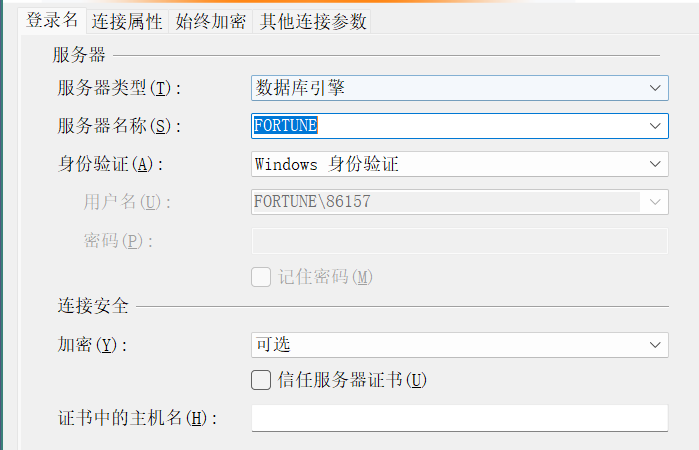
\includegraphics[width=0.7\textwidth]{img/1.png}
    \caption{SQL Server 管理员登录界面}
\end{figure}
\end{itemize}

\textbf{步骤1.2：创建SQL Server登录账户}

\begin{lstlisting}[language=SQL]
USE master;
GO

IF EXISTS (SELECT 1 FROM sys.server_principals WHERE name = 'mafuquan2024')
    DROP LOGIN mafuquan2024;
GO

CREATE LOGIN mafuquan2024
    WITH PASSWORD = '123456',
    DEFAULT_DATABASE = JY,
    CHECK_EXPIRATION = OFF,
    CHECK_POLICY = OFF;
GO

SELECT 
    name AS 登录名,
    type_desc AS 类型,
    default_database_name AS 默认数据库,
    create_date AS 创建日期
FROM sys.server_principals
WHERE name = 'mafuquan2024';
\end{lstlisting}

\noindent 登录账户创建结果如下：
\begin{figure}[H]
    \centering
    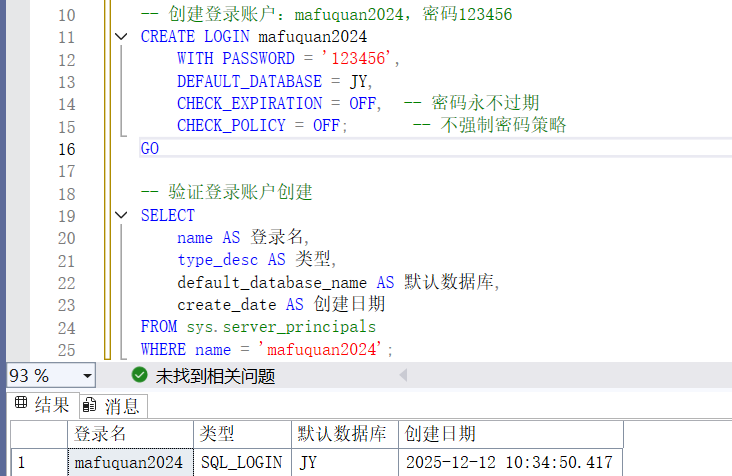
\includegraphics[width=0.7\textwidth]{img/2.png}
    \caption{登录账户创建结果}
\end{figure}

\textbf{步骤1.3：创建数据库用户}

\begin{lstlisting}[language=SQL]
USE JY;
GO

IF EXISTS (SELECT 1 FROM sys.database_principals WHERE name = 'mafuquan2024')
    DROP USER mafuquan2024;
GO

CREATE USER mafuquan2024 FOR LOGIN mafuquan2024;
GO

SELECT 
    name AS 用户名,
    type_desc AS 类型,
    authentication_type_desc AS 认证类型,
    default_schema_name AS 默认架构
FROM sys.database_principals
WHERE name = 'mafuquan2024';
\end{lstlisting}

\noindent 数据库用户创建结果如下：
\begin{figure}[H]
    \centering
    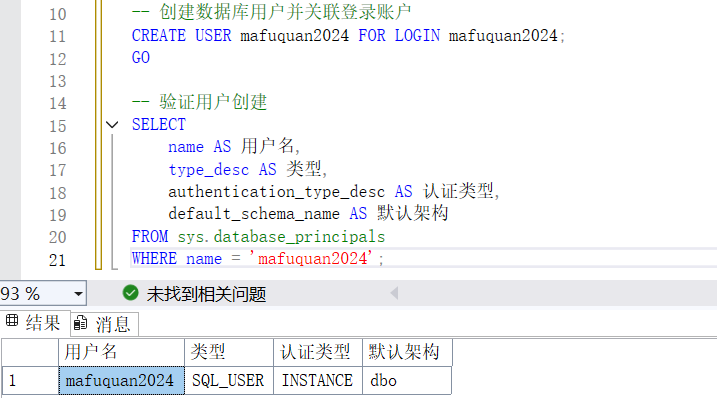
\includegraphics[width=0.7\textwidth]{img/3.png}
    \caption{数据库用户创建结果}
\end{figure}

\subsection{实验2：测试新用户权限}

\textbf{步骤2.1：断开当前连接，使用新账户登录}

\begin{itemize}
    \item 登录名：mafuquan2024，密码：123456
    \item 登录界面如图所示：
\begin{figure}[H]
    \centering
    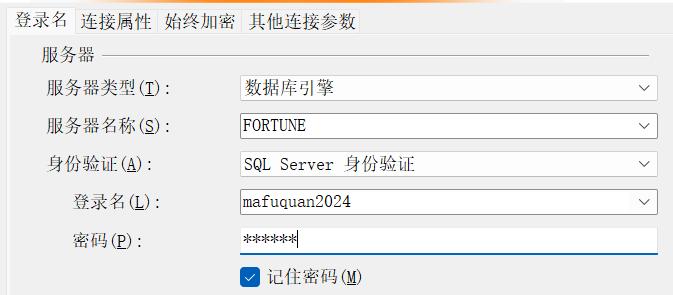
\includegraphics[width=0.7\textwidth]{img/4.png}
    \caption{新用户登录界面}
\end{figure}
\end{itemize}

\textbf{步骤2.2：尝试查询book表}

\begin{lstlisting}[language=SQL]
SELECT TOP 5 * FROM book;
\end{lstlisting}

\noindent 查询结果如下：
\begin{figure}[H]
    \centering
    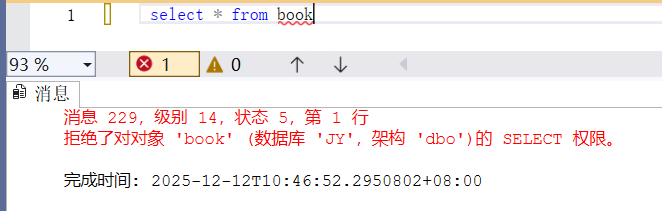
\includegraphics[width=0.7\textwidth]{img/5.png}
    \caption{新用户查询book表权限不足}
\end{figure}

如图所示，查询book表时出现权限不足的错误，说明新用户默认没有访问book表的权限。

\subsection{实验3：授予book表操作权限}

\textbf{步骤3.1：以管理员身份授权}

\begin{lstlisting}[language=SQL]
USE JY;
GO

GRANT SELECT, INSERT, UPDATE, DELETE ON dbo.book TO mafuquan2024;
GO

SELECT 
    USER_NAME(grantee_principal_id) AS 用户名,
    OBJECT_NAME(major_id) AS 对象名,
    permission_name AS 权限,
    state_desc AS 状态
FROM sys.database_permissions 
WHERE USER_NAME(grantee_principal_id) = 'mafuquan2024'
    AND OBJECT_NAME(major_id) = 'book';
\end{lstlisting}

\noindent 授权结果如下：
\begin{figure}[H]
    \centering
    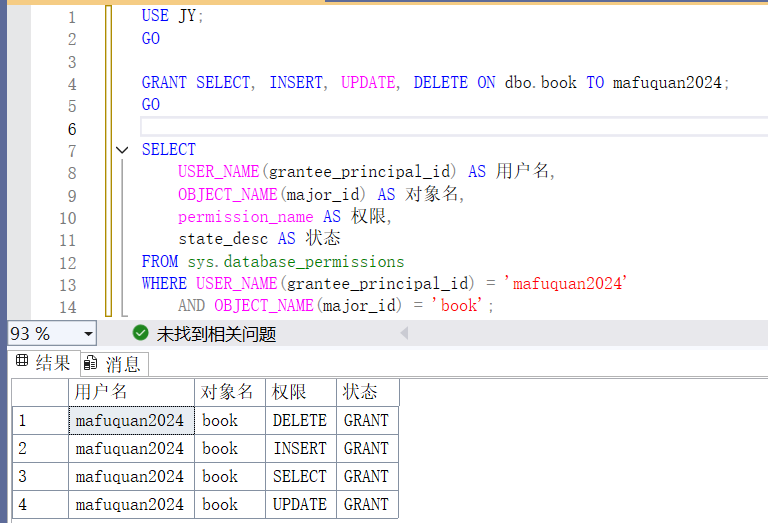
\includegraphics[width=0.7\textwidth]{img/6.png}
    \caption{book表权限授权结果}
\end{figure}

\textbf{步骤3.2：测试权限}

\begin{lstlisting}[language=SQL]
USE JY;
GO

-- SELECT权限
SELECT TOP 1 * FROM book;

-- INSERT权限
INSERT INTO book (book_id,book_isbn, book_name, book_author,book_price,book_publisher,interviews_times) 
VALUES ('t0001','978-7-121-22013-5', '权限测试图书',  '马福泉',99.99, '中山大学出版社',666);

-- UPDATE权限
UPDATE book 
SET book_name = '修改后的测试图书' 
WHERE book_id = 'TEST001';

-- DELETE权限
DELETE FROM book 
WHERE book_id = 'TEST001';

EXEC sp_helprotect @username = 'mafuquan2024';
\end{lstlisting}

\noindent 测试结果如下：
\begin{figure}[H]
    \centering
    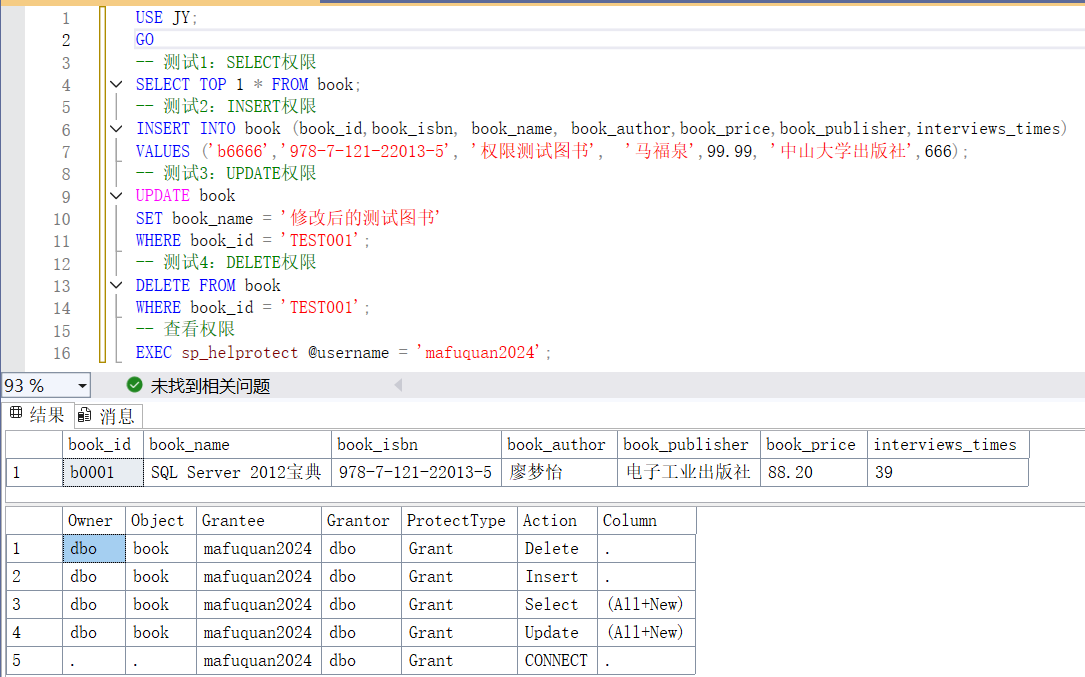
\includegraphics[width=0.6\textwidth]{img/7.png}
    \caption{book表操作权限测试（1）}
\end{figure}

\begin{figure}[H]
    \centering
    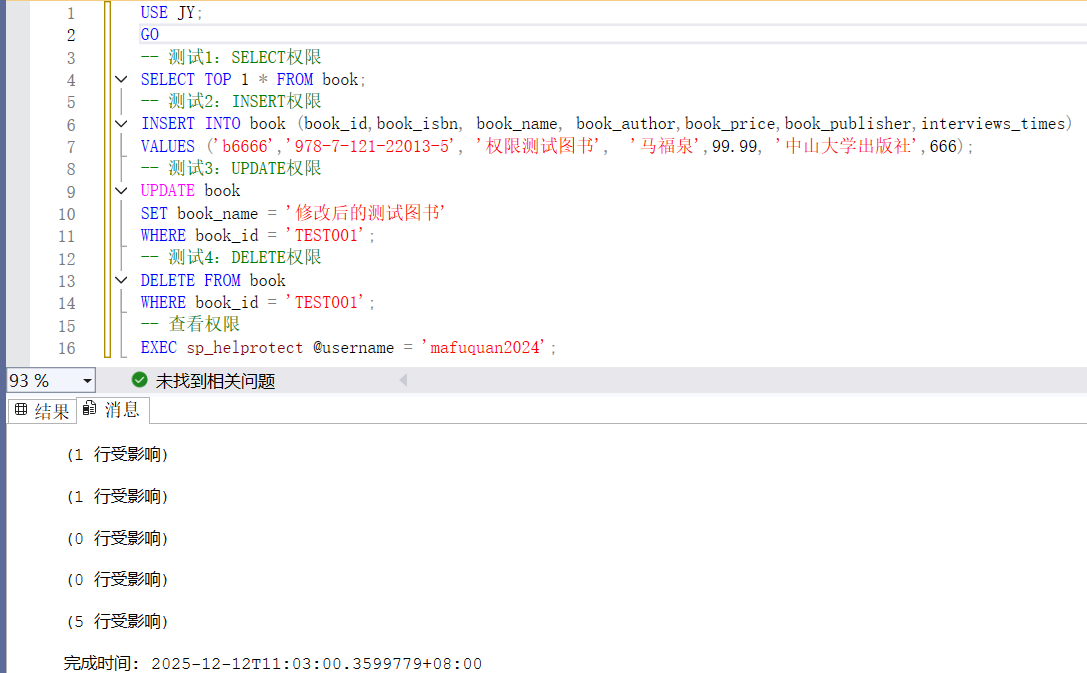
\includegraphics[width=0.6\textwidth]{img/8.png}
    \caption{book表操作权限测试（2）}
\end{figure}

如上图所示，用户mafuquan2024成功执行了SELECT、INSERT、UPDATE和DELETE操作，说明权限授予成功。

\subsection{实验4：撤销部分权限}

\textbf{步骤4.1：撤销UPDATE和DELETE权限}

\begin{lstlisting}[language=SQL]
USE JY;
GO

REVOKE UPDATE ON dbo.book FROM mafuquan2024;
REVOKE DELETE ON dbo.book FROM mafuquan2024;
GO

SELECT 
    USER_NAME(grantee_principal_id) AS 用户名,
    permission_name AS 权限,
    state_desc AS 状态
FROM sys.database_permissions 
WHERE USER_NAME(grantee_principal_id) = 'mafuquan2024'
    AND OBJECT_NAME(major_id) = 'book';
\end{lstlisting}

\noindent 权限撤销结果如下：
\begin{figure}[H]
    \centering
    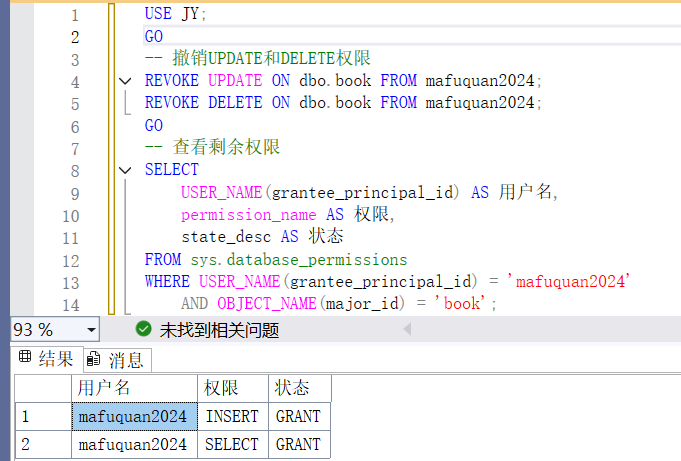
\includegraphics[width=0.7\textwidth]{img/9.png}
    \caption{撤销UPDATE和DELETE权限结果}
\end{figure}

\textbf{步骤4.2：测试撤销效果}

\begin{lstlisting}[language=SQL]
SELECT TOP 3 * FROM book;

INSERT INTO book (book_id,book_isbn, book_name, book_author,book_price,book_publisher,interviews_times) 
VALUES ('b6668','978-7-121-22013-5', '权限测试图书2',  '马福泉',99.99, '中山大学出版社',667);

BEGIN TRY
    UPDATE book 
    SET book_name = '尝试修改' 
    WHERE book_id = 'TEST002';
BEGIN CATCH
    PRINT 'UPDATE失败（预期结果）';
    PRINT ERROR_MESSAGE();
END CATCH

BEGIN TRY
    DELETE FROM book WHERE book_id = 'TEST002';
END TRY
BEGIN CATCH
    PRINT 'DELETE失败（预期结果）';
    PRINT ERROR_MESSAGE();
END CATCH
\end{lstlisting}

\noindent 测试结果如下：
\begin{figure}[H]
    \centering
    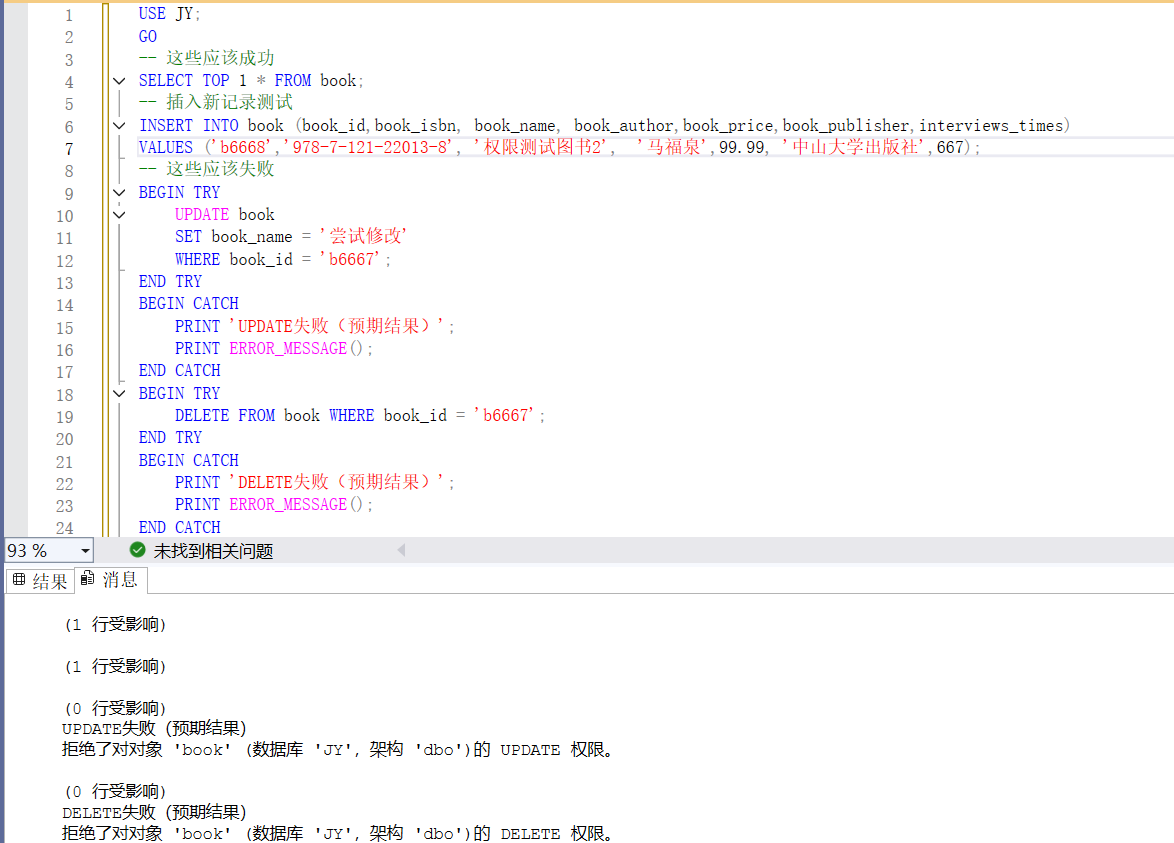
\includegraphics[width=0.7\textwidth]{img/10.png}
    \caption{撤销权限后操作测试结果}
\end{figure}

如上图，Select和Insert操作成功，而Update和Delete操作均失败，符合预期，说明权限撤销生效。

\subsection{实验5：创建视图并管理权限}

\textbf{步骤5.1：创建借阅次数$>$1的读者视图}

\begin{lstlisting}[language=SQL]
USE JY;
GO

CREATE VIEW dbo.v_reader_borrow_more_than_one
AS
SELECT 
    r.reader_id,
    r.reader_name,
    r.reader_sex,
    r.reader_department,
    COUNT(rec.borrow_date) AS borrow_count
FROM dbo.reader r
LEFT JOIN dbo.record rec ON r.reader_id = rec.reader_id
GROUP BY r.reader_id, r.reader_name, r.reader_sex, r.reader_department
HAVING COUNT(rec.borrow_date) > 1;
GO

SELECT TOP 10 * FROM dbo.v_reader_borrow_more_than_one
ORDER BY borrow_count DESC;
\end{lstlisting}

\noindent 视图创建及查询结果如下：
\begin{figure}[H]
    \centering
    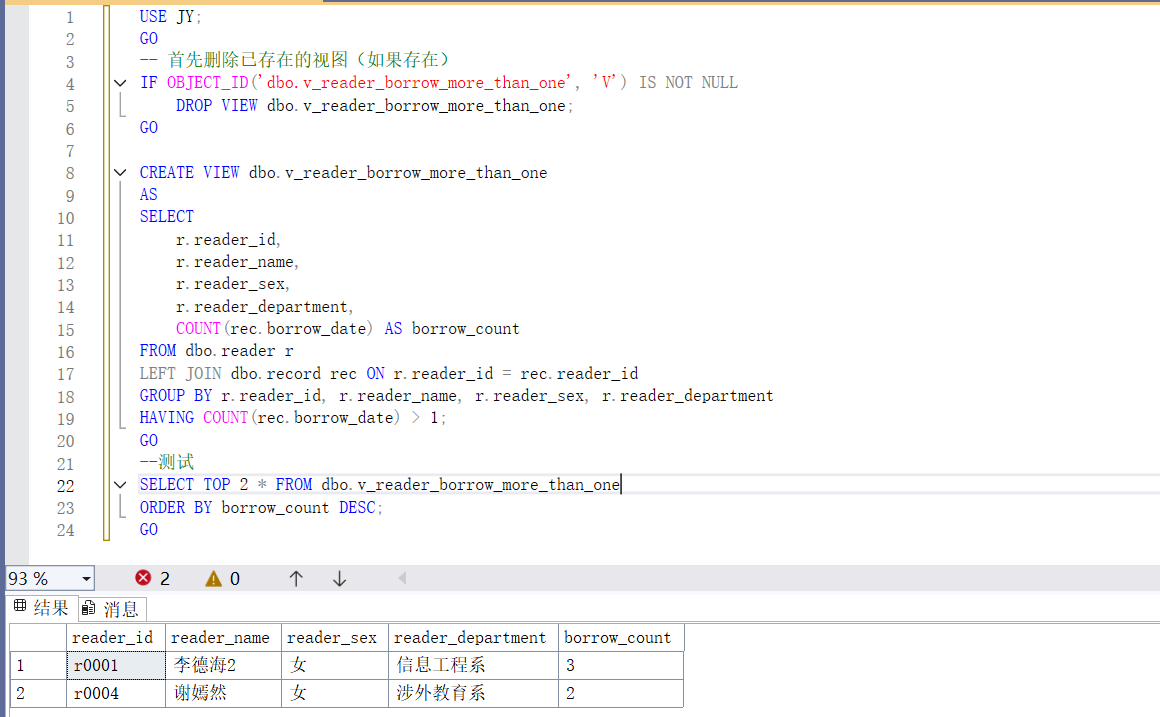
\includegraphics[width=0.7\textwidth]{img/11.png}
    \caption{借阅次数大于1的读者视图及查询结果}
\end{figure}

\textbf{步骤5.2：授予视图SELECT权限}

\begin{lstlisting}[language=SQL]
GRANT SELECT ON dbo.v_reader_borrow_more_than_one TO mafuquan2024;
GO

SELECT 
    USER_NAME(grantee_principal_id) AS 用户名,
    OBJECT_NAME(major_id) AS 对象名,
    permission_name AS 权限
FROM sys.database_permissions 
WHERE USER_NAME(grantee_principal_id) = 'mafuquan2024'
    AND OBJECT_NAME(major_id) = 'v_reader_borrow_more_than_one';
\end{lstlisting}

\noindent 授权结果如下：
\begin{figure}[H]
    \centering
    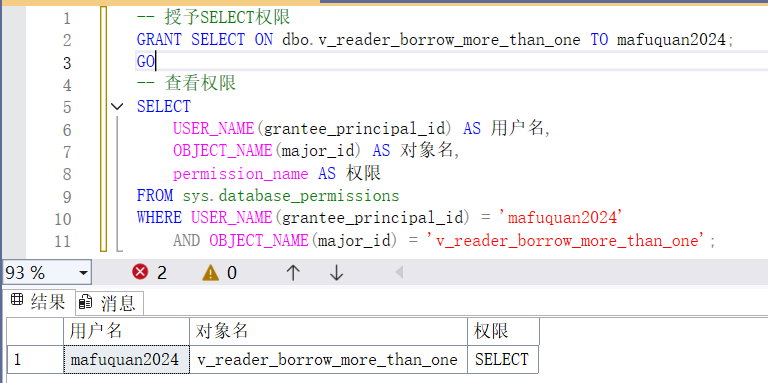
\includegraphics[width=0.7\textwidth]{img/12.png}
    \caption{视图SELECT权限授权结果}
\end{figure}

\textbf{步骤5.3：测试视图访问}

\begin{lstlisting}[language=SQL]
USE JY;
GO
SELECT TOP 10 * FROM v_reader_borrow_more_than_one
ORDER BY borrow_count DESC;
\end{lstlisting}

\noindent 查询结果如下：
\begin{figure}[H]
    \centering
    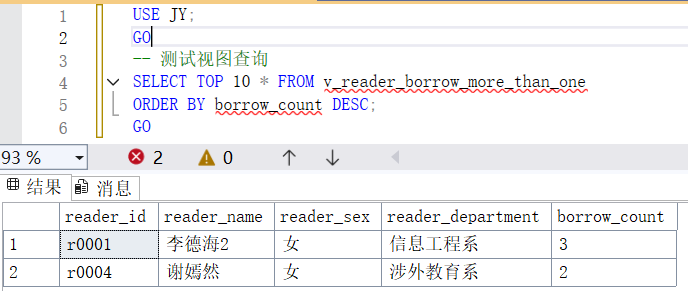
\includegraphics[width=0.7\textwidth]{img/14.png}
    \caption{新用户访问视图查询结果}
\end{figure}
如上图所示，用户mafuquan2024成功查询了视图，说明SELECT权限授予成功。

\textbf{步骤5.4：撤销视图权限}

\begin{lstlisting}[language=SQL]
USE JY;
GO

REVOKE SELECT ON dbo.v_reader_borrow_more_than_one FROM mafuquan2024;
GO

IF NOT EXISTS (
    SELECT 1 
    FROM sys.database_permissions 
    WHERE USER_NAME(grantee_principal_id) = 'mafuquan2024'
        AND OBJECT_NAME(major_id) = 'v_reader_borrow_more_than_one'
)
    PRINT '权限已成功撤销';
\end{lstlisting}

\noindent 权限撤销结果如下：
\begin{figure}[H]
    \centering
    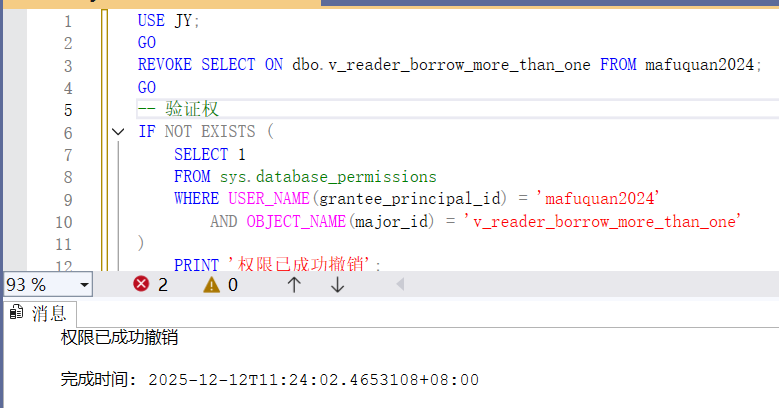
\includegraphics[width=0.7\textwidth]{img/15.png}
    \caption{撤销视图权限结果}
\end{figure}

\subsection{实验6：创建部门限制视图}

\textbf{步骤6.1：检查reader表数据}

\begin{lstlisting}[language=SQL]
SELECT DISTINCT reader_department, COUNT(*) as 人数
FROM reader
GROUP BY reader_department
ORDER BY reader_department;
\end{lstlisting}

\textbf{步骤6.2：创建“涉外教育系”读者视图}

\begin{lstlisting}[language=SQL]
IF OBJECT_ID('dbo.v_reader_foreign_edu', 'V') IS NOT NULL
    DROP VIEW dbo.v_reader_foreign_edu;
GO

CREATE VIEW dbo.v_reader_foreign_edu
AS
SELECT 
    reader_id,
    reader_name,
    reader_sex,
    reader_department
FROM dbo.reader
WHERE reader_department = N'涉外教育系';
GO

SELECT * FROM dbo.v_reader_foreign_edu;
\end{lstlisting}

\noindent 视图创建及查询结果如下：
\begin{figure}[H]
    \centering
    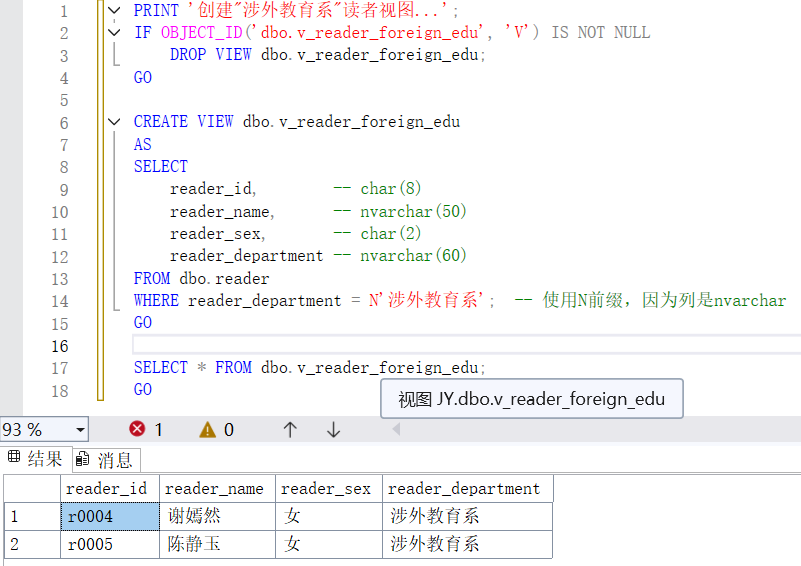
\includegraphics[width=0.7\textwidth]{img/16.png}
    \caption{“涉外教育系”读者视图及查询结果}
\end{figure}

\textbf{步骤6.3：查看权限}

\begin{lstlisting}[language=SQL]
SELECT 
    USER_NAME(grantee_principal_id) AS 用户名,
    permission_name AS 权限,
    state_desc AS 状态
FROM sys.database_permissions 
WHERE USER_NAME(grantee_principal_id) = 'mafuquan2024'
    AND OBJECT_NAME(major_id) = 'v_reader_foreign_edu';
\end{lstlisting}

\noindent 权限结果如下：
\begin{figure}[H]
    \centering
    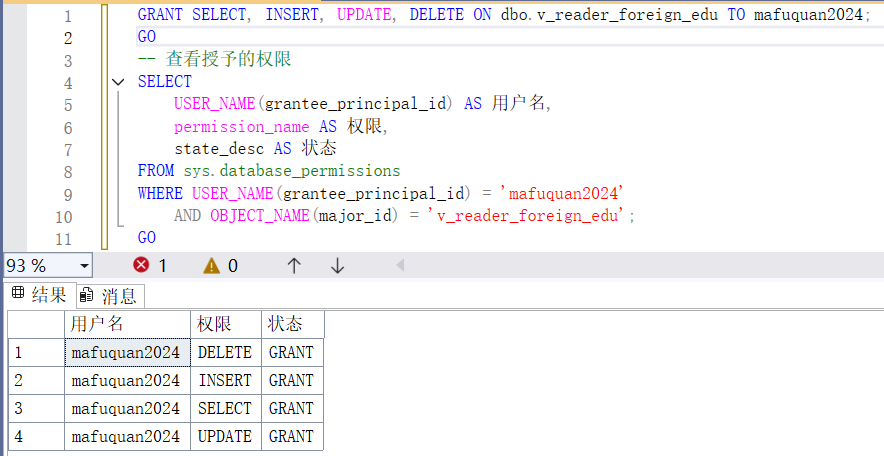
\includegraphics[width=0.7\textwidth]{img/17.png}
    \caption{“涉外教育系”视图权限结果}
\end{figure}

\textbf{步骤6.4：测试视图所有权限}

\begin{lstlisting}[language=SQL]
-- 1. SELECT测试
SELECT TOP 3 * FROM v_reader_foreign_edu;
GO
-- 2. INSERT测试
INSERT INTO v_reader_foreign_edu (reader_id, reader_name, reader_sex, reader_department)
VALUES ('R666999', N'测试外教读者', N'女', N'涉外教育系');
GO
-- 3. UPDATE测试
UPDATE v_reader_foreign_edu 
SET reader_name = N'修改后的外教读者' 
WHERE reader_id = 'R666999';
GO
-- 4. DELETE测试
DELETE FROM v_reader_foreign_edu WHERE reader_id = 'R666999';
GO
-- 5. 测试跨部门插入
INSERT INTO v_reader_foreign_edu (reader_id, reader_name, reader_sex, reader_department)
VALUES ('CROSS001', N'其他系读者', N'男', N'信息工程系');
GO
\end{lstlisting}

\noindent 权限及操作结果如下：
\begin{figure}[H]
    \centering
    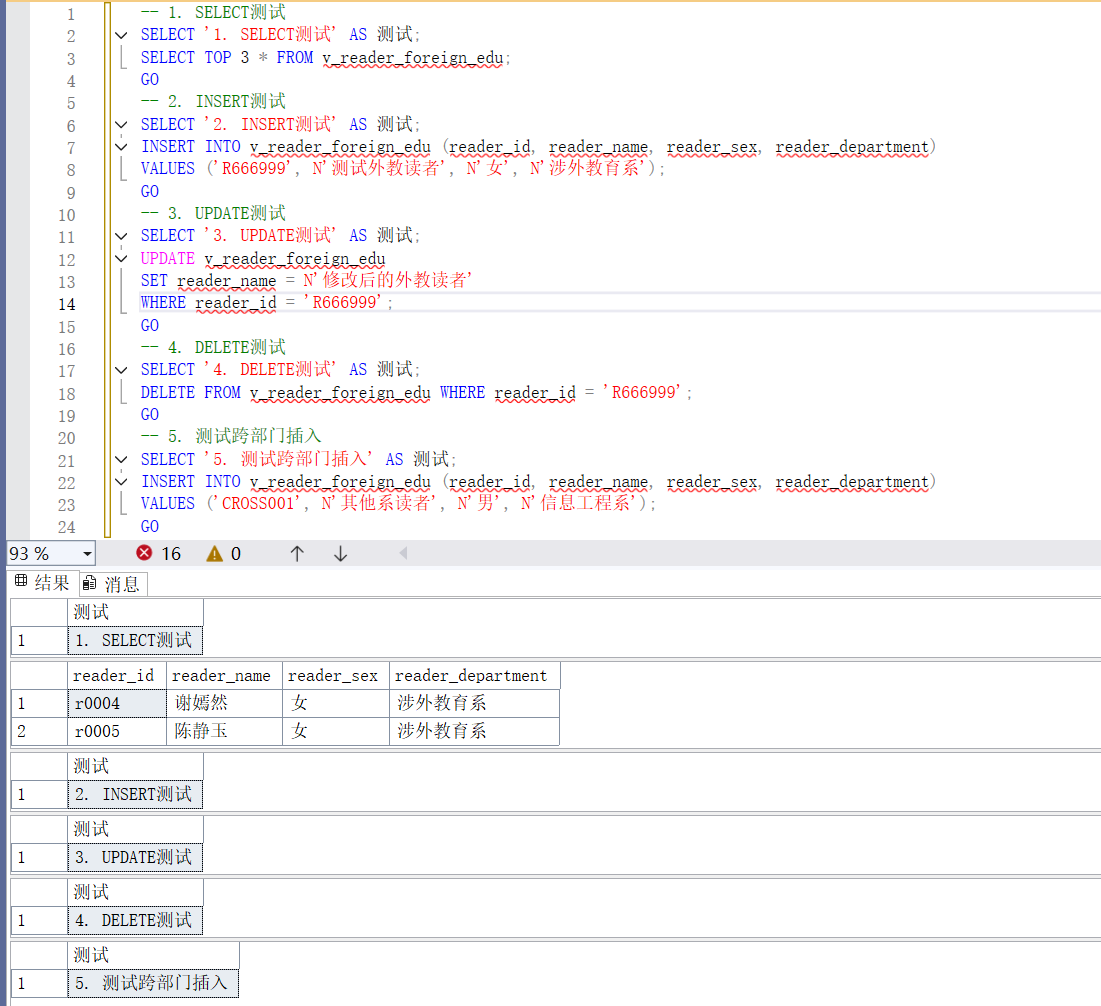
\includegraphics[width=0.7\textwidth]{img/18.png}
    \caption{“涉外教育系”视图权限及操作测试结果}
\end{figure}
如上图所示，用户mafuquan2024成功执行了SELECT、INSERT、UPDATE和DELETE操作，且无法插入非“涉外教育系”的读者数据，说明视图权限设置正确。

\subsection{实验总结}

\subsubsection{困难和解决}
在实验过程中遇到如下主要困难及解决办法：

\textbf{困难：连接到服务器时出现证书链错误}
\begin{itemize}
    \item \textbf{问题描述：}  
    在使用SQL Server Management Studio连接服务器“FORTUNE”时，出现如下报错：

    \begin{quote}
    标题: 连接到服务器
    无法连接到 FORTUNE。
    其他信息:
    A connection was successfully established with the server, but then an error occurred during the login process. (provider: SSL Provider, error: 0 - 证书链是由不受信任的颁发机构颁发的。) (Microsoft SQL Server，错误: -2146893019)
    证书链是由不受信任的颁发机构颁发的。
    \end{quote}

    \item \textbf{解决方案：}  
    在登录窗口的“其他连接参数”选项卡中，添加如下参数：
    \begin{lstlisting}
TrustServerCertificate=True
    \end{lstlisting}
    这样即可跳过证书信任校验，顺利连接到服务器。
\end{itemize}

\subsubsection{主要收获}
通过本次实验，初步理解了SQL Server数据库的安全性控制机制，掌握了以下技能：
\begin{itemize}
    \item 能够创建SQL Server登录账户和数据库用户，理解两者的区别与联系；
    \item 熟悉了数据库对象（如表、视图）的权限分配与回收操作；
    \item 熟悉了常见权限错误的排查与验证流程。
\end{itemize}
\end{document}